\documentclass[9pt]{beamer}
\usepackage{minted}
%\usemintedstyle{manni}
\usemintedstyle{murphy}
\usepackage{hyperref}
\hypersetup{
colorlinks=true,
urlcolor=blue
}
\usepackage{graphicx}

\begin{document}
\title{Basic Introduction to gcloud}
\author{Nick Thompson} 
\date{\today}

\frame{\titlepage}

\begin{frame}[fragile]
  \frametitle{Goals of this discussion}
  \pause
  \begin{itemize}
  \item Learn how to rent CPUs and RAM from google
    \pause
  \item Learn how to rent persistent disks
    \pause
  \item Learn how to control expenses
    \pause
  \item Learn how to manage permissions
    \pause
  \item Learn how to create teams of identical VMs
    \pause
  \item Learn how to autoscale nodes based on load
  \end{itemize}
\end{frame}

\begin{frame}[fragile]
  \frametitle{What we won't discuss, but should}
  \pause
  \begin{itemize}
  \item The Python/Go/Node bindings
    \pause
  \item The REST (representational state transfer) interface
    \pause
  \item gcloud sql
  \end{itemize}
\end{frame}

\begin{frame}[fragile]
\frametitle{Getting started:}
\begin{minted}{bash}
 $ curl https://sdk.cloud.google.com | bash
  $ exec -l $SHELL
  $ gcloud init
  $ gcloud auth login
  $ firefox https://console.developers.google.com
\end{minted}
You don't need a gmail account to use gcloud, but you must enter an email into gcloud that then becomes your google account login.
\end{frame}

\begin{frame}[fragile]
  \frametitle{Starting a Project}
  \begin{figure}
    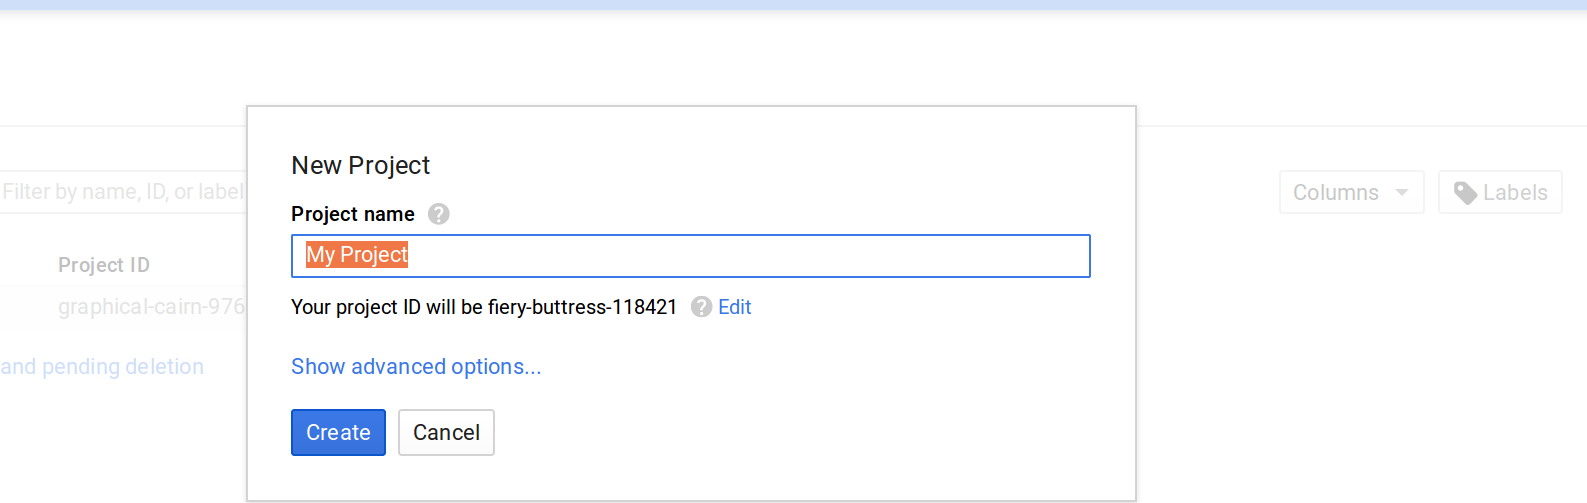
\includegraphics[scale=0.2]{figures/CreateProject.png}
  \end{figure}
\end{frame}

\begin{frame}[fragile]
  \frametitle{Starting a Project}
  Each project has
  \pause
  \begin{itemize}
  \item its bill separated in the invoice (1 billing account $\mapsto$ many project accounts)
    \pause
  \item its own VMs
    \pause
  \item its own persistent disks
    \pause
  \item its own users with their associated permissions.
  \end{itemize}
\end{frame}

\begin{frame}[fragile]
  \frametitle{Starting a Project}
  Multiple people can be listed as project owners, or given read access, or read/write access to the project:
  \begin{figure}
    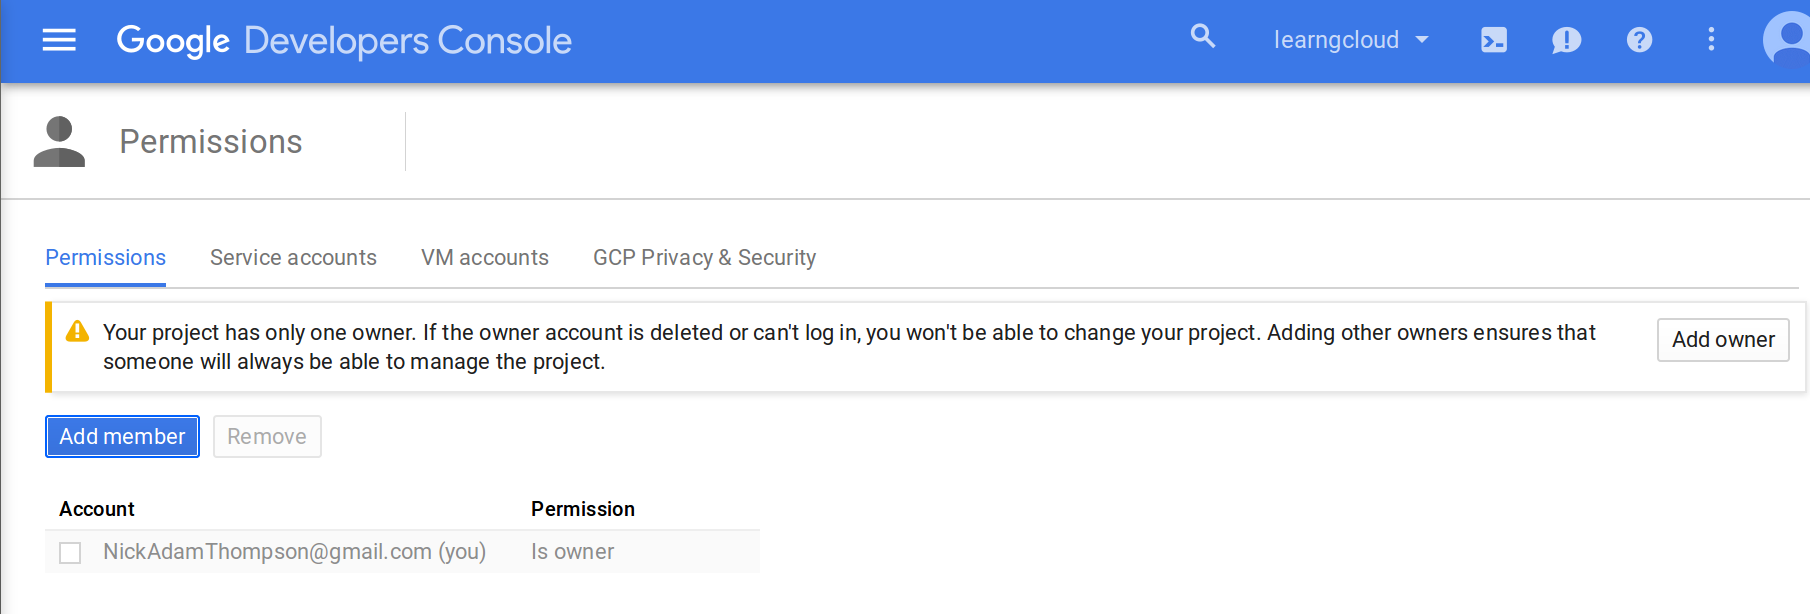
\includegraphics[scale=0.2]{figures/AddProjectOwner.png}
  \end{figure}
  \emph{Note that people who only have read access to the project nonetheless have root access to all the VMs!}
\end{frame}

\begin{frame}[fragile]
  \frametitle{Starting a Project}
  When you grant someone permission to view/edit/co-own your project, they receive an email asking them if they want to join:
  \begin{figure}
    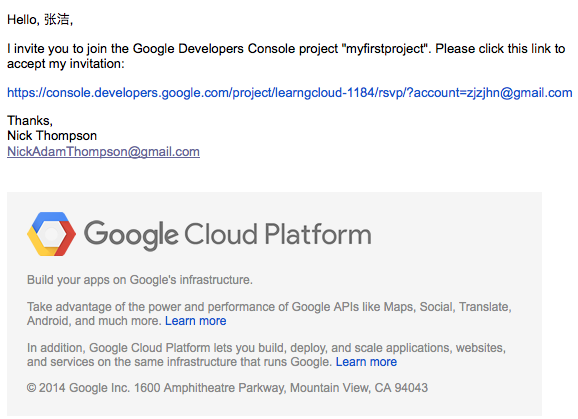
\includegraphics[scale=0.4]{figures/EmailConfirmation.png}
  \end{figure}
\end{frame}

\begin{frame}[fragile]
  \frametitle{gcloud user accounts}
  gcloud user accounts are in beta, and seem to be evolving rapidly. To see more, use
  \begin{minted}{bash}
$ gcloud beta compute users -h
  \end{minted}
or visit the \href{https://cloud.google.com/compute/docs/access/user-accounts/}{docs}.
\end{frame}

\begin{frame}[fragile]
  \frametitle{Starting a project}
  You need tell the gcloud command-line tool that you've created a new project:
  \begin{minted}{bash}
    $ gcloud config list
    [core]
    account = nickadamthompson@gmail.com
    disable_usage_reporting = True
    project = graphical-cairn-97618 
    [meta]
    active_config = default
  \end{minted}
  If the \texttt{project} field has the wrong value, you need to set it:
  \begin{minted}{bash}
    $ gcloud config set project learngcloud-1184
  \end{minted}
  Note that you don't set the project \emph{name}, you set the project \emph{ID}.
\end{frame}


\begin{frame}[fragile]
  \frametitle{Setting up an instance}
  \begin{figure}
    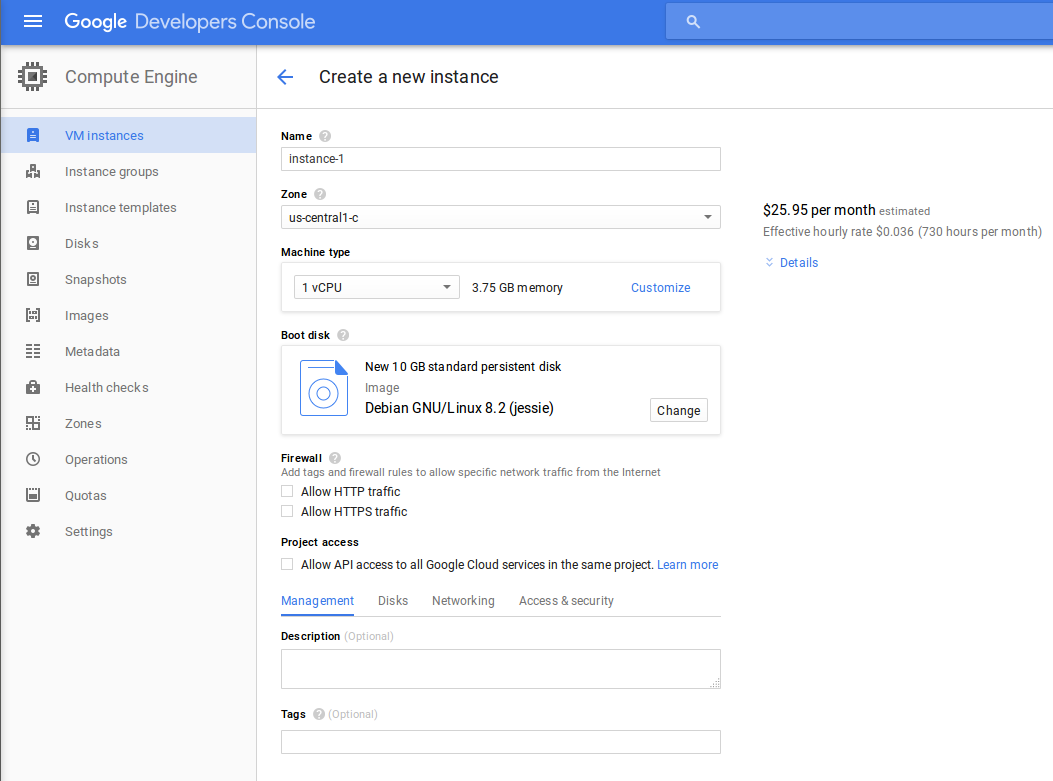
\includegraphics[scale=0.3]{figures/CreateInstance.png}
  \end{figure}
\end{frame}

\begin{frame}[fragile]
  \frametitle{Setting up an instance}
  Things to choose at this point:
  \pause
  \begin{itemize}
  \item Number of cores (max 32)
    \pause
  \item amount of RAM (unlimited, it seems, but 200GB is supported for sure)
    \pause
  \item size of disk, SSD (max 10TB) or spinning (max 10TB) 
    \pause
  \item Operating system (Ubuntu, Centos, CoreOS), or choose a VM snapshot
    \pause
  \item Firewall rules
    \pause
  \item Whether to use static or ephemeral IP addresses (static IPs cost money!)
  \end{itemize}
\end{frame}

\begin{frame}[fragile]
  \frametitle{Setting up an instance}
  Aside: If you need more than 10TB of disk space, you need to fill out the \href{https://docs.google.com/a/google.com/forms/d/1vb2MkAr9JcHrp6myQ3oTxCyBv2c7Iyc5wqIKqE3K4IE/viewform}{Google Compute Engine Quota Change Request Form}.
\end{frame}

\begin{frame}[fragile]
  \frametitle{Setting up an instance}
  Once you create a VM, you'll be assigned an external IP address and can see the load on your server:
  \begin{figure}
    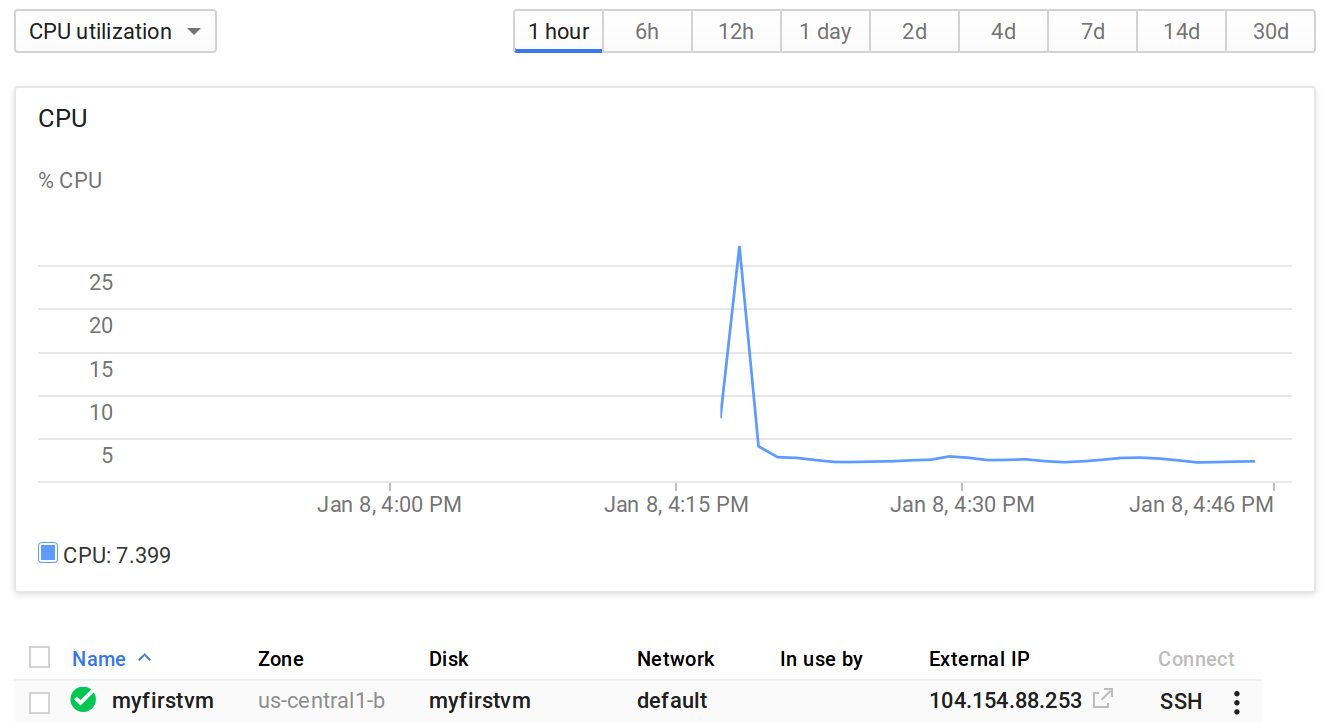
\includegraphics[scale=0.2]{figures/VMUp.png}
  \end{figure}
\end{frame}

\begin{frame}[fragile]
  \frametitle{Setting up an instance}
  To access your VM, use:
  \begin{minted}{bash}
    $ gcloud compute ssh myfirstvm --zone us-central1-b
  \end{minted}
  (Don't choose the wrong zone or else your instance won't be found!)

  This is really a wrapper script around the IP address of your instance:
  \begin{minted}{bash}
    $ ssh -i ~/.ssh/google_compute_engine 104.154.88.253
  \end{minted}
\end{frame}

\begin{frame}[fragile]
  \frametitle{Setting up an instance}
  For every console action, there is a equivalent gcloud command. So, for example, to set up an instance, you could type
  \begin{minted}{bash}
    $ gcloud compute instances create mysecondvm \
         --image ubuntu-15-10 --zone us-central1-b
  \end{minted}
  This is useful for scripting.
\end{frame}

\begin{frame}[fragile]
  \frametitle{Snapshotting an instance}
  Once you have installed your favorite software on your VM, you might want to snapshot it:
  \begin{minted}{bash}
myfirstvm$ sudo apt-get update
myfirstvm$ sudo apt-get install -y gcc g++ emacs git
myfirstvm$ sudo touch /opt/hello.txt && sudo chmod a+rw /opt/hello.txt
myfirstvm$ echo "Hello from GCE!" >> /opt/hello.txt
myfirstvm$ exit
localhost$ gcloud compute disks snapshot "myfirstvm" \
              --zone "us-central1-b" --snapshot-names "firstvmsnapshot"
  \end{minted}  
\end{frame}

\begin{frame}[fragile]
  \frametitle{Snapshotting an instance}
  Of course, using the console GUI is a bit easier:
  \begin{figure}
    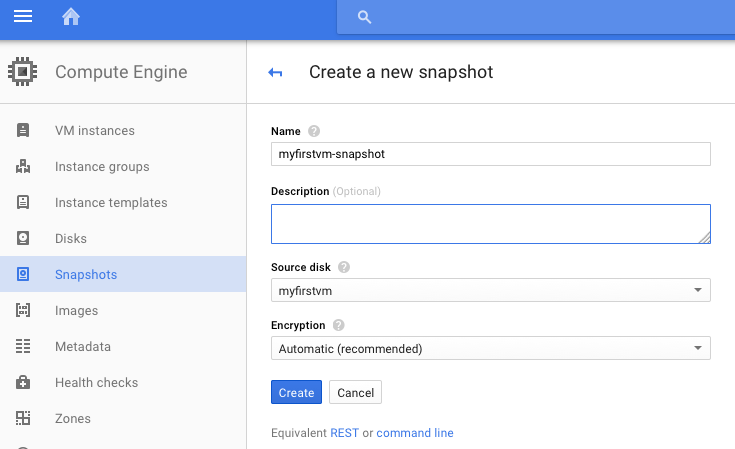
\includegraphics[scale=0.3]{figures/SnapshotVM.png}
  \end{figure}
\end{frame}

\begin{frame}[fragile]
  \frametitle{Snapshotting an instance}
  Once you have a snapshot, you can create a boot disk from it:
\begin{figure}
  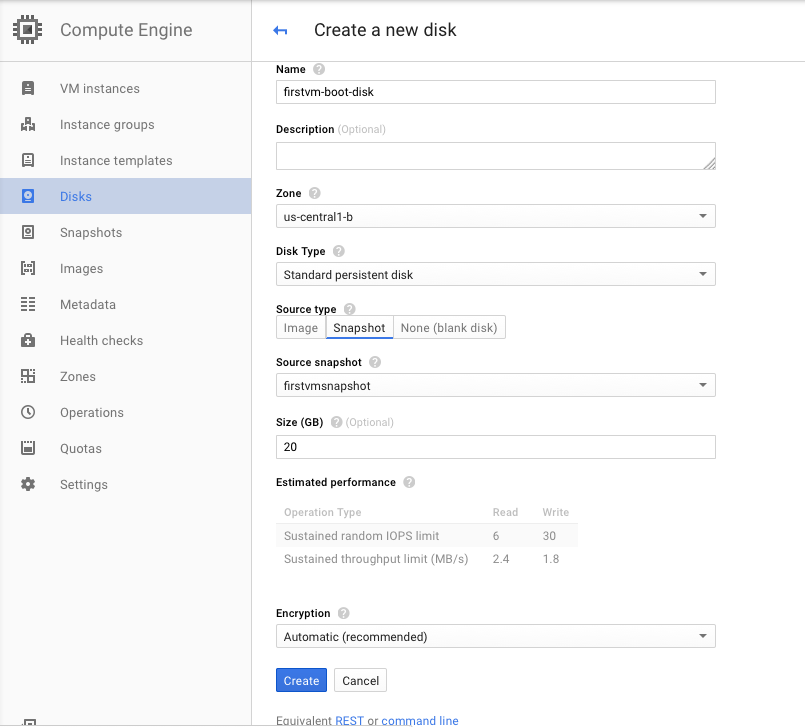
\includegraphics[scale=0.3]{figures/BootDisk.png}
\end{figure}
\end{frame}

\begin{frame}[fragile]
  \frametitle{Snapshotting an instance}
  And once you have a boot disk, you can create a VM from it:
  \begin{figure}
    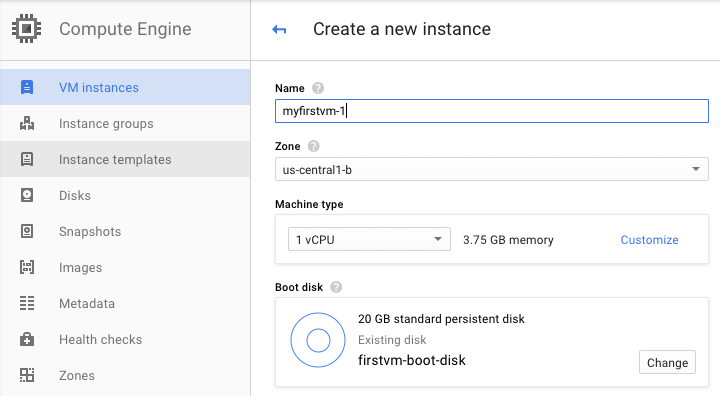
\includegraphics[scale=0.3]{figures/VMFromBootDisk.png}
  \end{figure}
\end{frame}

\begin{frame}[fragile]
  \frametitle{Replicating VMs}
  A boot disk can only be attached in RW mode to a single instance. To attach a boot disk in read-only mode to many instances, use
  \begin{minted}{bash}
$ gcloud compute instances create vm-{1..3} --zone us-central1-b \
   --disk name=firstvm-boot-disk,boot=yes,mode=ro
  \end{minted}
\end{frame}

\begin{frame}[fragile]
  \frametitle{Regions and Zones}
  Google divides the world into regions:
  \begin{minted}{bash}
$ gcloud compute regions list
NAME         CPUS          DISKS_GB     ADDRESSES RESERVED_ADDRESSES STATUS TURNDOWN_DATE
asia-east1      0.00/24.00     10/10240      0/23      0/7           UP
europe-west1    0.00/24.00      0/10240      0/23      0/7           UP
us-central1     4.00/24.00     40/10240      4/23      0/7           UP
us-east1        0.00/24.00      0/10240      0/23      0/7           UP
  \end{minted}
\end{frame}

\begin{frame}[fragile]
  \frametitle{Regions and Zones}
  And each region is divided into multiple zones
\begin{minted}{bash}
$ gcloud compute zones list
NAME           REGION       STATUS NEXT_MAINTENANCE TURNDOWN_DATE
asia-east1-a   asia-east1   UP
asia-east1-b   asia-east1   UP
asia-east1-c   asia-east1   UP
europe-west1-b europe-west1 UP
europe-west1-d europe-west1 UP
europe-west1-c europe-west1 UP
us-central1-c  us-central1  UP
us-central1-a  us-central1  UP
us-central1-f  us-central1  UP
us-central1-b  us-central1  UP
us-east1-c     us-east1     UP
us-east1-b     us-east1     UP
us-east1-d     us-east1     UP
\end{minted}
\end{frame}

\begin{frame}[fragile]
  \frametitle{Regions and Zones}
  A zone is essentially single datacenter, so two instances in a zone can communicate very quickly with one another:
  \begin{minted}{bash}
    vmcentral1b-1$ ping vmcentral1b-2 # ping VM in same datacenter/zone:
    rtt min/avg/max/mdev = 0.308/0.394/0.841/0.104 ms
    vmcentral1b-1$ ping vmcentral1a # Ping VM in same region, different zone:
    rtt min/avg/max/mdev = 0.571/0.673/1.210/0.099 ms
    vmcentral1b-1$ ping vm-in-asia 
    rtt min/avg/max/mdev = 154.738/154.878/155.326/0.442 ms
  \end{minted}
  So within-zone communication is fastest, within-region is fast, between-region is slow. (Note how your instance names are resolved via DNS!)
\end{frame}

\begin{frame}[fragile]
  \frametitle{Editing Firewalls}
  Google cloud has a set of default firewall rules that you might like to edit:
  \begin{figure}
    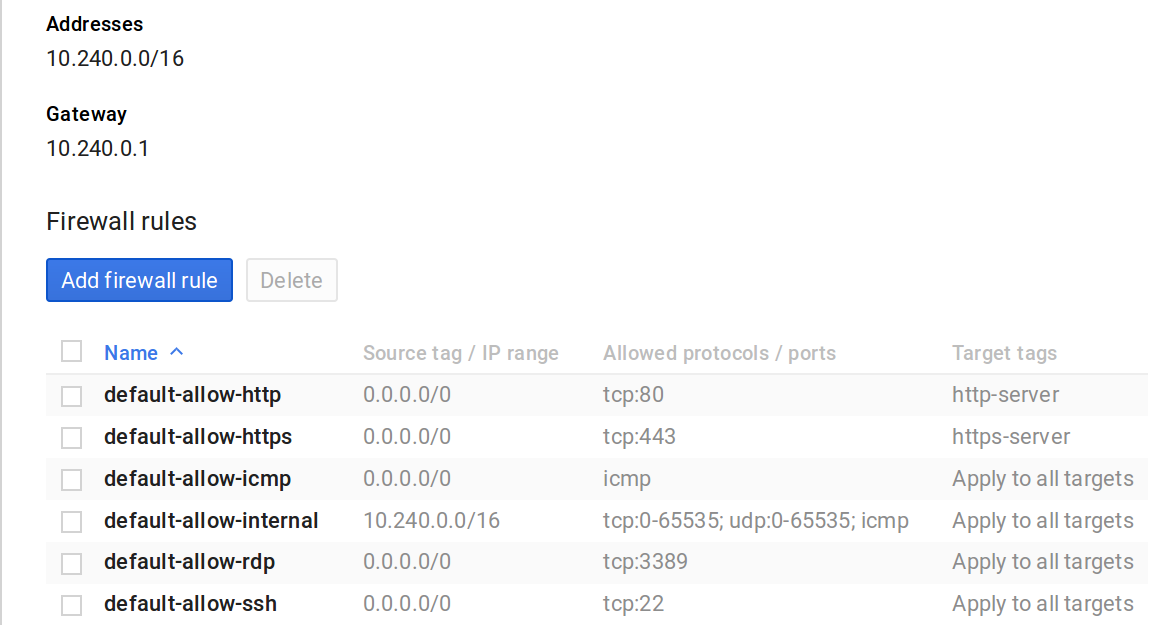
\includegraphics[scale=0.2]{figures/DefaultFirewall.png}
  \end{figure}
\end{frame}

\begin{frame}[fragile]
Note that all ports are available via the internal ip addresses 10.240.0.0/16
  \begin{minted}{bash}
$ gcloud compute firewall-rules list
NAME                   NETWORK SRC_RANGES    RULES                        SRC_TAGS TARGET_TAGS
default-allow-http     default 0.0.0.0/0     tcp:80                                http-server
default-allow-https    default 0.0.0.0/0     tcp:443                               https-server
default-allow-icmp     default 0.0.0.0/0     icmp
default-allow-internal default 10.240.0.0/16 tcp:0-65535,udp:0-65535,icmp
default-allow-ssh      default 0.0.0.0/0     tcp:22    
  \end{minted}

\end{frame}

\begin{frame}[fragile]
  \frametitle{Editing Firewalls}
  The default rules are of course reflected in the port scan:
  \begin{minted}{bash}
    $ nmap -p 0-10000 104.154.88.253

    Starting Nmap 6.47 ( http://nmap.org ) at 2016-01-08 17:43 CST
    Nmap scan report for 253.88.154.104.bc.googleusercontent.com (104.154.88.253)
    Host is up (0.040s latency).
    Not shown: 9997 filtered ports
    PORT     STATE  SERVICE
    22/tcp   open   ssh
    80/tcp   closed http
    443/tcp  closed https
    3389/tcp closed ms-wbt-server
  \end{minted}
\end{frame}

\begin{frame}[fragile]
  \frametitle{Editing firewalls}
  This allows traffic from AMQP:
  \begin{figure}
    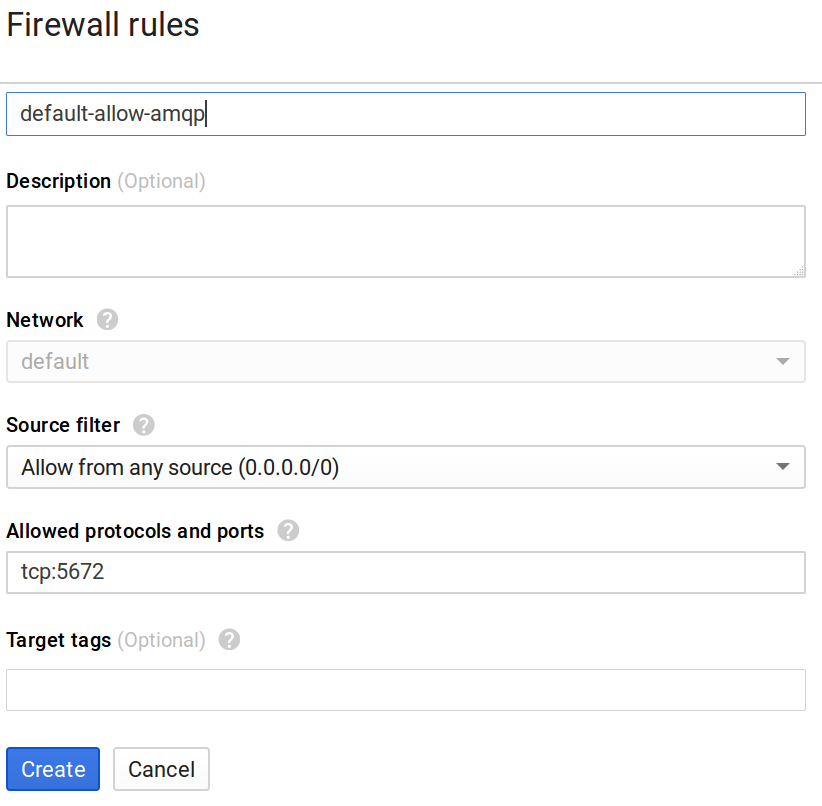
\includegraphics[scale=0.2]{figures/DefineFirewall.png}
  \end{figure}
\end{frame}

\begin{frame}[fragile]
  \frametitle{Editing firewalls}
  Command line to allow AMQP on port 5672 from any source IP, use the command
  \begin{minted}{bash}
    $ gcloud compute firewall-rules create default-allow-amqp --allow tcp:5672
    Created [https://www.googleapis.com/compute/v1/projects/learngcloud-1184/global/firewalls/default-allow-amqp].
    NAME               NETWORK SRC_RANGES RULES    SRC_TAGS TARGET_TAGS
    default-allow-amqp default 0.0.0.0/0  tcp:5672
  \end{minted}
  Creating a firewall rule applies it to all live instances in the project.
\end{frame}

\begin{frame}[fragile]
  \frametitle{Networking}
  Each project supports a $2^{16} = 65,536$ address internal network:
  \begin{minted}{bash}
$ gcloud compute networks list
NAME    IPV4_RANGE    GATEWAY_IPV4
default 10.240.0.0/16 10.240.0.1    
  \end{minted}
\end{frame}

\begin{frame}[fragile]
  \frametitle{Load balancing}
  Let's set up a couple servers to learn how to load balance:
  \begin{minted}{bash}
$ gcloud compute instances create httpserver1 --tags frontend --zone us-central1-a
$ gcloud compute firewall-rules create http-frontend --allow tcp:80 --target-tags frontend
$ gcloud compute ssh httpserver1
httpserver1$ sudo apt-get update && sudo apt-get install -y nginx
httpserver1$ sudo emacs /var/www/html/index.nginx-debian.html 
  \end{minted}
Edit the file so that it tells us what server it comes from; do the same for httpserver2.
\end{frame}

\begin{frame}[fragile]
  \frametitle{Load Balancing}
  Now let's set up a ``target-pool'', a group of server that responds to requests:
\begin{minted}{bash}
$ gcloud compute target-pools create frontends --region us-central1
$ gcloud compute target-pools add-instances frontends --instances httpserver1 --zone us-central1-a
$ gcloud compute target-pools add-instances frontends --instances httpserver2 --zone us-central1-b
$ gcloud compute forwarding-rules create frontends --target-pool frontends --region us-central1
NAME      REGION      IP_ADDRESS     IP_PROTOCOL TARGET
frontends us-central1 104.154.36.151 TCP         us-central1/targetPools/frontends
$ for i in {1..100}; do curl 104.154.36.151; done
Welcome to httpserver2!
Welcome to httpserver1!
Welcome to httpserver2!
Welcome to httpserver2!
Welcome to httpserver1!
\end{minted}
\end{frame}


\begin{frame}[fragile]
  \frametitle{Persistent Disks}
  If you need storage that is not chained to a particular VM, then you need to use ``buckets'':
  \begin{figure}
    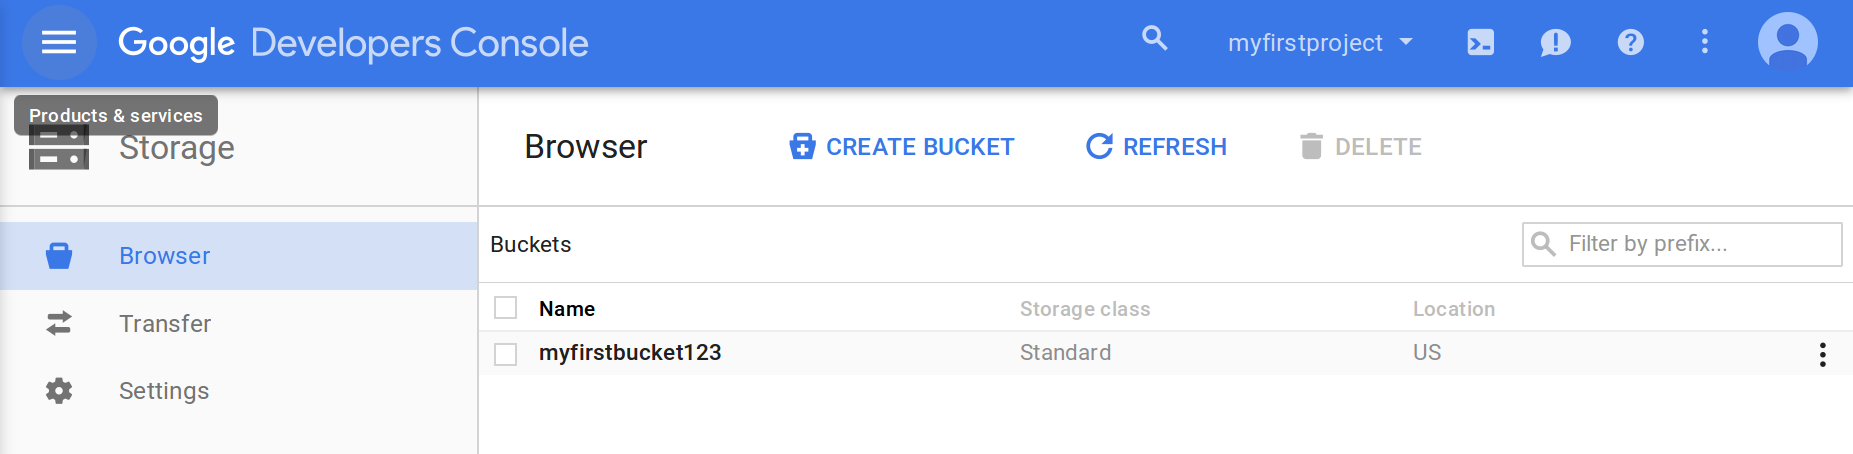
\includegraphics[scale=0.2]{figures/Buckets.png}
  \end{figure}
\end{frame}

\begin{frame}[fragile]
  \frametitle{Persistent Disks}
  In order to manage persistent disks from the command line, use the gsutil utility:
  \begin{minted}{bash}
    $ pip install gsutil
    $ gsutil mb gs://myfirstbucket
    Creating gs://myfirstbucket/...
    ServiceException: 409 Bucket myfirstbucket already exists.
    $ gsutil mb gs://myfirstbucket123
    Creating gs://myfirstbucket123/...
    $ gsutil cp talk.log gs://myfirstbucket123
    Copying file://talk.log [Content-Type=application/octet-stream]...
    Uploading   gs://myfirstbucket123/talk.log:                      43.94 KiB/43.94 KiB
    ~/learn_gcloud$ gsutil ls
    gs://myfirstbucket123/
    $ gsutil ls -l gs://myfirstbucket123
    44993  2016-01-09T21:19:30Z  gs://myfirstbucket123/talk.log
    TOTAL: 1 objects, 44993 bytes (43.94 KiB)
  \end{minted}
  Bucket names need to be globally unique across all of gcloud!
\end{frame}

\begin{frame}[fragile]
  \frametitle{Persistent Disks}
  \begin{itemize}
  \item gcloud buckets are encrypted on disk
  \item gcloud buckets are accessible outside zones
  \item Uploads to gcloud buckets are atomic and considered successful once the info is stored in multiple datacenters.
  \item BLOBs in buckets \emph{cannot be edited}. They can be overwritten, however.
  \end{itemize}
\end{frame}

\begin{frame}[fragile]
  \frametitle{Persistent Disks}
  Mounting a bucket to an instance takes a little work (\href{https://github.com/googlecloudplatform/gcsfuse/blob/master/docs/installing.md}{instructions}):
\begin{minted}{bash}
$ curl -L -O https://github.com/GoogleCloudPlatform/gcsfuse/releases/download/v0.15.0/gcsfuse_0.15.0_amd64.deb
$ sudo dpkg --install gcsfuse_0.15.0_amd64.deb
$ mkdir mount_point
$ gcsfuse myfirstbucket123 mount_point
$ time ls mount_point
  talk.log
  real0m2.557s
$ touch mount_point/file.txt
touch: cannot touch ‘mount_point/file.txt’: Input/output error
\end{minted}
  These networked disks are \emph{incredibly slow}, even read-only.
\end{frame}

\begin{frame}[fragile]
  \frametitle{Persistent Disks}
  A few more \texttt{gsutil} examples:
  \begin{minted}{bash}
$ gsutil rsync gs://myfirstbucket123/  `pwd`
Building synchronization state...
Starting synchronization
Copying gs://myfirstbucket123/talk.log...
Downloading file:///home/NAThompson/talk.log:                    43.94 KiB/43.94 KiB
$ gsutil rsync `pwd` gs://myfirstbucket123/foo
Building synchronization state...
Starting synchronization
...
$ gsutil du -h gs://myfirstbucket123
43.94 KiB   gs://myfirstbucket123/talk.log
  \end{minted}
\end{frame}

\begin{frame}[fragile]
  \frametitle{Persistent Disks}
  The need to access to persistent disks via APIs in various languages is very common. gcloud has Python, Node.js, Java, and Ruby bindings. Let's see an example in Python:
  \begin{minted}{python}
    $ pip3 install git+https://github.com/GoogleCloudPlatform/gcloud-python.git
    $ python3 -q
    >>> from gcloud import storage
    >>> client = storage.Client(project='learngloud-1184', credentials='')
  \end{minted}
\end{frame}

\begin{frame}[fragile]
  \frametitle{References}
  \begin{itemize}
  \item \href{http://www.amazon.com/Google-Compute-Engine-Marc-Cohen/dp/1449360882/ref=sr_1_1?ie=UTF8&qid=1452552286&sr=8-1&keywords=Google+Compute+Engine}{Google Compute Engine}, by Marc Cohen, Kathryn Hurley, and Paul Newson
  \item \href{http://www.amazon.com/Building-Thing-Google-Cloud-Platform/dp/1484210050/ref=pd_sim_14_2?ie=UTF8&dpID=51NfTEhpFlL&dpSrc=sims&preST=_AC_UL160_SR11\%2C160_&refRID=1XA05PG1Q6D5NW63685Y}{Building Your Next Big Thing With Google Cloud Platform}, by Jose Gonzales and S. Krishnan.
  \end{itemize}
\end{frame}

\end{document}
